\documentclass{llncs}% ===> this file was generated automatically by noweave --- better not edit it
\usepackage{epsfig}
\usepackage{noweb}
\pagestyle{noweb}
\noweboptions{}
\begin{document}
\nwfilename{userguide.nw}
\title{BREW: Breakable web application for lectures in IT-Security}
\author{C Pohl 
\\ \email{christoph.pohl0@hm.edu}}
\institute{Department for Computer Sciences and Mathematics\\ University of Applied Sciences\\ Munich}
\maketitle

\nwbegindocs{0}
\begin{figure}
\centering

\includegraphics[width=1\textwidth]{logo}
\end{figure}
\section{Introduction or how to read this file}
This file looks a bit strange. There are a lot of references and broken source code. And there are some fancy references like {\Tt{}\LA{}README~{\nwtagstyle{}\subpageref{NW4Ugr3m-1u9106-1}}\RA{}\nwendquote}.

At first this document (and big parts of BREW) are written in literate programming. This means you will write a documentation which includes the source code (normally you write source code and a documentation for it..). Even the makefile to generate the documentation is included in the documentation...However this is a nitty gritty way to write source code, it will also produce some uncommon documentation. To read this paper you just need to know that there are references like this {\Tt{}\LA{}README~{\nwtagstyle{}\subpageref{NW4Ugr3m-1u9106-1}}\RA{}\nwendquote}. This means that there is a reference to a codechunk (a piece of code). This occurs in code chunks or in plain text. The liitle number at the end of such a reference is the page where this code is located in this document. In every code block there are one or two references. One on the left side. This is the label for this piece of code. On the right side you will find a reference to former code. 

Give it a try and find the {\Tt{}\LA{}README~{\nwtagstyle{}\subpageref{NW4Ugr3m-1u9106-1}}\RA{}\nwendquote} code in this document. Than watch the README in the source directory. This is the tangling output from literate programming. Also look at the different sourcefiles, including the {\Tt{}\LA{}Makefile~{\nwtagstyle{}\subpageref{nw@notdef}}\RA{}\nwendquote} and the \LaTeX sources. Everything is build from the original {\em userguide.nw}.

However this is a nice way to write well documented code. In the source folder you can find the full source code, including the {\Tt{}\LA{}Makefile~{\nwtagstyle{}\subpageref{nw@notdef}}\RA{}\nwendquote} to recreate BREW, this document and even the html version. You will need a few tools for this. At first you will need Latex, noweb (for the literate programming part), gcc, make, java and python. But this is a bit out of scope now.

\section{BREW in a virtual machine}
\subsection{Some basics}
It is not necessary to use BREW in a virtual machine. BREW is just a simple web application and a bit of source code in your IDE.
However, you can use the preconfigured virtual machine. 

In the most cases you will use the VirtualBox environment (You can also use KVM-qemu which is the cool way, but not really a handy solution. The KVM-qemu machine is meant for the use in a cloud environment). At first copy the .ova file. You can also test this file against the provided hashsum (You should do this if you choosed to download the full package). Howver find a suitable space in your directory and copy the .ova in this directory. Then you need to import your virtual machine. (Use import virtual machine). All the fancy configuration should be done automatically (It is preconfigured). However there are a few possible problems there. 

\begin{itemize}
\item You need write access to the directory (Really you have to read the error statements. This is one of the most common problems in lectures...)
\item You need sufficient space
\item You need a 64 Bit operating system
\item You need the VT flag enabled
\end{itemize} 

OK what is VT flag? Read some manuals (or just google)...

OK what is 64 Bit? You are computer scientist...

Sounds trivial? OK it is! Read carefully the error messages, in most cases you will find one of the errors above....

How to deal with it? Ask your admin or use google....

\subsection{Some important notes for configuration}
The virtual machine is preconfigured, when you want to adopt the system to your needs read the prerequisites (c.f. Table \ref{tab:prereq}) for the guest machine.

\begin{table}
\centering
\caption{Owasp Top Ten Attacks}
\label{tab:prereq}
\begin{tabular}{llllll}
\hline\noalign{\smallskip}
Prerequisite & value\\
\noalign{\smallskip}
\hline
\noalign{\smallskip}
RAM & 512 MB\\
IO-APIC & True\\
Processor & 1\\
PAE-NX & False\\
VT-X/AMD-V & True\\
Graphic Ram & 9MB\\
Network & Host only or NAT(Never Bridged...really dangerous)\\
\hline
\end{tabular}
\end{table}
Hence the most common configuration will be RAM (whatever you want) and processor (whatever you want). This will enhance the performance.

Never ever use a bridged network. BREW is a vulnerable web application. This means it is really vulnerable (no game). With a bridged network you will expose BREW to the rest of the world (or your local lan). 

\subsection{Start BREW and beyond}
After successful import just press start in VirtualBox. The virtual machine will start and after a few seconds you will see a nice looking and well designed terminal (c.f. Figure \ref{fig:login})...

\begin{figure}
\centering
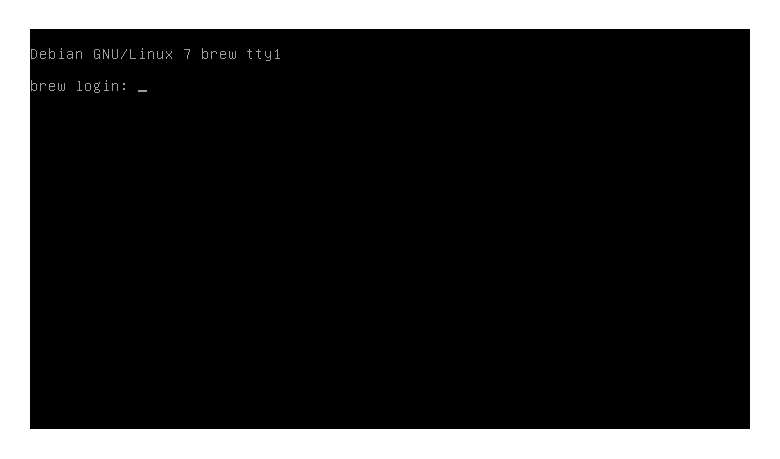
\includegraphics[width=1\textwidth]{screenshot_start}
\caption{Screenshot login} 
\label{fig:login}
\end{figure}

To log in use {\Tt{}username:muse\nwendquote} and {\Tt{}password:muse\nwendquote}. You can also login with {\Tt{}root:muse\nwendquote}. By the way, just the normal muse user has a functional X-Server configuration.
In normal cases you should see something like in Figure \ref{fig:loginsuc}

\begin{figure}
\centering
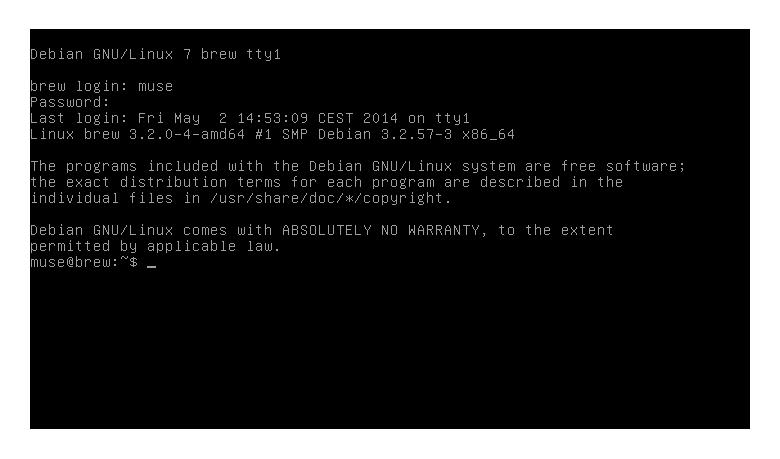
\includegraphics[width=1\textwidth]{screenshot_loggedin}
\caption{Screenshot login successful} 
\label{fig:loginsuc}
\end{figure}

However this is nice and you are ready to start a successful career with BREW. A real nerd does not need to use stuff like the X-Server. In this moment you can use BREW just with vim and some nice console commands.

However, we had too much complaints about the usability, we implemented openbox for your convenience.

To start the X-Server type {\Tt{}startx\nwendquote} in the command line.
However when everything is ok, you should see something like in Figure \ref{fig:brewwork}

\begin{figure}
\centering
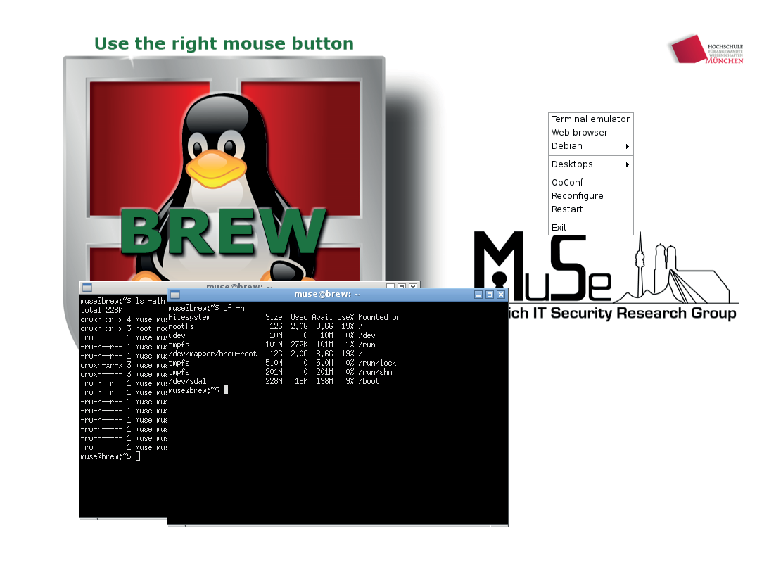
\includegraphics[width=1\textwidth]{running_brew}
\caption{BREW works} 
\label{fig:brewwork}
\end{figure}

\section{BREW in the IDE}
BREW can be started directly from the IDE. For this you need to open the project. Do not import, extract or try other unfancy things. Just open the project. You can do this with {\em File$\rightarrow$Open} from the IDE. Sounds trivial but in every lecture this is a common error...
In the case of the virtual machine, you just need to open eclipse. The project is the default project.

However you will find some nitty gritty hints in the README file. Hence this guide is written in literate programming, the README file is generated out of this document...
But is also part of this document (fancy or?). The file is in the appendix {\Tt{}\LA{}README~{\nwtagstyle{}\subpageref{NW4Ugr3m-1u9106-1}}\RA{}\nwendquote}.

In the {\Tt{}\LA{}README~{\nwtagstyle{}\subpageref{NW4Ugr3m-1u9106-1}}\RA{}\nwendquote} you will find all necessary tips for a successful exercise.

As proposed in the {\Tt{}\LA{}README~{\nwtagstyle{}\subpageref{NW4Ugr3m-1u9106-1}}\RA{}\nwendquote} there is a mainfile. This mainfile is proposed under {\Tt{}\LA{}TomcatServer.java~{\nwtagstyle{}\subpageref{NW4Ugr3m-38m9kp-1}}\RA{}\nwendquote}.
When you want to change the port for BREW you can do this in this main file.

\section{Architectural basics}
\subsection{Database and Webserver}
The database is an embedded hlsql database. It always renews whenever BREW gets restarted. There is no persistent storage. 

The webserver is an embedded Tomcat. It gets started whenever BREW gets started. Hence a webserver needs a listening address and port you can not start more than one server on one port...Typically you get an exception 

{\Tt{}...\nwnewline
java.net.BindException:\ Address\ already\ in\ use\ <null>:8081\nwnewline
...\nwendquote}

This exception occurs whenever more than one server is bound to the same port. However this happens when you have a running instance and try to debug...

\subsection{Important pathes}
In BREW there are two important pathes for the exercises. The pathes are easy to find with the knowledge about the structure. As proposed in \ref{subsec:controller} one must find the controller and the corresponding view. Simplified at first one must look at the functionality. Each functionality (p.Ex search) has a mapping Controller (p.Ex. SearchController.java). Just look on the page in BREW, and you will find immediatly the corresponding controller. Another part of interest is the view. The view is calculated with the viewname. Simplified with {\Tt{}viewname+".jsp"\nwendquote}. In BREW you can find the controller and view on different places.
The controller are under {\em src$\rightarrow$edu$\rightarrow$hm$\rightarrow$muse$\rightarrow$controller}, the views are within {\em webapps$\rightarrow$secu$\rightarrow$WEB-INF$\rightarrow$pages}
 

\subsection{Controller overview}\label{subsec:controller}
The architecture integrates a classical MVC pattern to provide the web application.As underlying framework the widely used Spring framework is sued. The Spring framework is a lightweight platform for java applications. For the sake of simplicity, the focus is set on the vulnerabilities. A schematic overview is given in Figure \ref{fig:architecture}

\begin{figure}
\centering
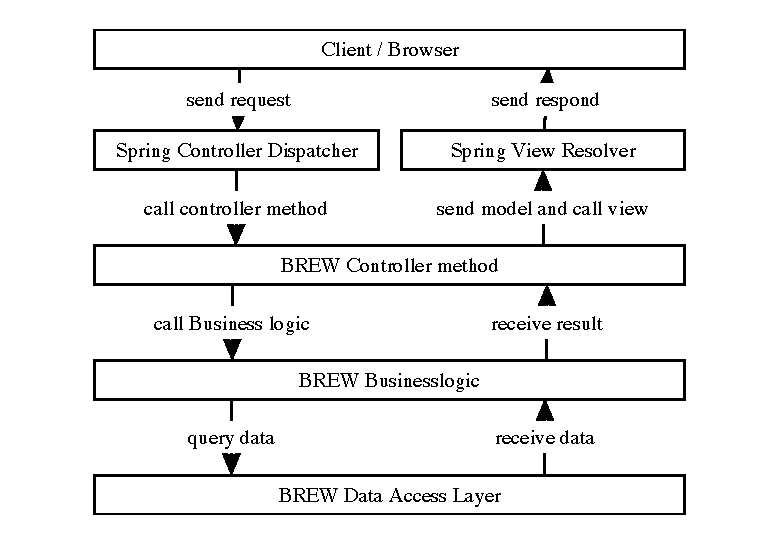
\includegraphics[width=1\textwidth]{architecture_fin}
\caption{BREW architecture} 
\label{fig:architecture}
\end{figure}

At first the browser send an request to BREW. Within the path matching of the Springframework a controller method gets called. In this example the search page is mapped to {\em http://mydomain/search.secu}. For simplicity every logical component has a related controller class (p.Ex. {\em Searchpage $\rightarrow$ SearchController.java}). Every action within this logical component inherits a method. (p.Ex {\em search $\rightarrow$ searchWebWithPost($\dots$)}).
Within this method the Businesslogic occurs. The businesslogic can ask the data access layer. This logic produces a HashMap-based model for further usage in the related view. In this example, the view gets the variable {\em search} accessible with the key {\em searchString}.


\subsection{Some basics to the Controller}
The Controller is just a simple javafile. It consists on different parts. Hence this is written in literate programming, we need to explain everything....
\nwfilename{userguide.nw}\nwbegincode{1}\sublabel{NW4Ugr3m-4fUKe6-1}\nwmargintag{{\nwtagstyle{}\subpageref{NW4Ugr3m-4fUKe6-1}}}\moddef{SearchController.java~{\nwtagstyle{}\subpageref{NW4Ugr3m-4fUKe6-1}}}\endmoddef\nwstartdeflinemarkup\nwenddeflinemarkup
\LA{}some fancy license stuff~{\nwtagstyle{}\subpageref{NW4Ugr3m-M1MOe-1}}\RA{}
\LA{}some import statements for the SearchController~{\nwtagstyle{}\subpageref{NW4Ugr3m-J2zL7-1}}\RA{}
\LA{}class declaration for search controller~{\nwtagstyle{}\subpageref{NW4Ugr3m-1a0CYJ-1}}\RA{}
        \LA{}method declaration for search controller~{\nwtagstyle{}\subpageref{NW4Ugr3m-2vmaBC-1}}\RA{}
\nwnotused{SearchController.java}\nwendcode{}\nwbegindocs{2}\nwdocspar
Hence it is trivial to define a class. There is an important annotation. This ensures that the Spring FRamework knows that this class acts like a controller.
\nwenddocs{}\nwbegincode{3}\sublabel{NW4Ugr3m-1a0CYJ-1}\nwmargintag{{\nwtagstyle{}\subpageref{NW4Ugr3m-1a0CYJ-1}}}\moddef{class declaration for search controller~{\nwtagstyle{}\subpageref{NW4Ugr3m-1a0CYJ-1}}}\endmoddef\nwstartdeflinemarkup\nwusesondefline{\\{NW4Ugr3m-4fUKe6-1}}\nwenddeflinemarkup
@Controller
public class SearchController \{
\nwused{\\{NW4Ugr3m-4fUKe6-1}}\nwendcode{}\nwbegindocs{4}\nwdocspar
A method for any controller is just a method. This method gets called by the dispatcher from spring. This depends on the URI and the parameter.
\nwenddocs{}\nwbegincode{5}\sublabel{NW4Ugr3m-2vmaBC-1}\nwmargintag{{\nwtagstyle{}\subpageref{NW4Ugr3m-2vmaBC-1}}}\moddef{method declaration for search controller~{\nwtagstyle{}\subpageref{NW4Ugr3m-2vmaBC-1}}}\endmoddef\nwstartdeflinemarkup\nwusesondefline{\\{NW4Ugr3m-4fUKe6-1}}\nwenddeflinemarkup
\LA{}Mapping for post based search action~{\nwtagstyle{}\subpageref{NW4Ugr3m-Bgkc9-1}}\RA{}
\LA{}declaration for post based search action method~{\nwtagstyle{}\subpageref{NW4Ugr3m-ir6Gd-1}}\RA{}
        \LA{}method body for post based seach action method~{\nwtagstyle{}\subpageref{NW4Ugr3m-hNOrN-1}}\RA{}
        
\nwused{\\{NW4Ugr3m-4fUKe6-1}}\nwendcode{}\nwbegindocs{6}\nwdocspar

The basic request mapping is done with the annotation over the corresponding method. This will map every request to the URI {\em http://mydomain/secu/search.secu} to this method. But only when the request method is {\em POST} and the parameters will match.
\nwenddocs{}\nwbegincode{7}\sublabel{NW4Ugr3m-Bgkc9-1}\nwmargintag{{\nwtagstyle{}\subpageref{NW4Ugr3m-Bgkc9-1}}}\moddef{Mapping for post based search action~{\nwtagstyle{}\subpageref{NW4Ugr3m-Bgkc9-1}}}\endmoddef\nwstartdeflinemarkup\nwusesondefline{\\{NW4Ugr3m-2vmaBC-1}}\nwenddeflinemarkup
@RequestMapping
        (value = "/search.secu", 
        method = RequestMethod.POST)
\nwused{\\{NW4Ugr3m-2vmaBC-1}}\nwendcode{}\nwbegindocs{8}\nwdocspar

The second mapping part is done over the matchin parameters. In this case there can be a parameter named {\em search}. The value for this parameter, p.Ex from a text input field will be present in the variable {\em search}. However if this parameter is not present, the variable will be null.
\nwenddocs{}\nwbegincode{9}\sublabel{NW4Ugr3m-ir6Gd-1}\nwmargintag{{\nwtagstyle{}\subpageref{NW4Ugr3m-ir6Gd-1}}}\moddef{declaration for post based search action method~{\nwtagstyle{}\subpageref{NW4Ugr3m-ir6Gd-1}}}\endmoddef\nwstartdeflinemarkup\nwusesondefline{\\{NW4Ugr3m-2vmaBC-1}}\nwenddeflinemarkup
public ModelAndView searchWebWithPost
        (@RequestParam
                (value = "search", 
                required = false) 
                String search) \{
\nwused{\\{NW4Ugr3m-2vmaBC-1}}\nwendcode{}\nwbegindocs{10}\nwdocspar

In normal cases the method body needs to return a Model and a View. In this body the business logic is called. The controller consists of different stages in model and view generation.
\nwenddocs{}\nwbegincode{11}\sublabel{NW4Ugr3m-hNOrN-1}\nwmargintag{{\nwtagstyle{}\subpageref{NW4Ugr3m-hNOrN-1}}}\moddef{method body for post based seach action method~{\nwtagstyle{}\subpageref{NW4Ugr3m-hNOrN-1}}}\endmoddef\nwstartdeflinemarkup\nwusesondefline{\\{NW4Ugr3m-2vmaBC-1}}\nwenddeflinemarkup
\LA{}generate searchmodel and view~{\nwtagstyle{}\subpageref{NW4Ugr3m-PiA1k-1}}\RA{}
\LA{}fill searchmodel with data~{\nwtagstyle{}\subpageref{NW4Ugr3m-KyitU-1}}\RA{}
\LA{}return model and view~{\nwtagstyle{}\subpageref{NW4Ugr3m-2aKjAb-1}}\RA{}
\}
\nwused{\\{NW4Ugr3m-2vmaBC-1}}\nwendcode{}\nwbegindocs{12}\nwdocspar
To generate a model and view there is a special type in Spring. The {\em ModelAndView} class combines the model and view. As parameter the name of the view is injected. In our case it is {\em search}. This maps to {\em search.jsp}. Hence the mapping is generated and simplify the suffix {\em .jsp} gets appended.
\nwenddocs{}\nwbegincode{13}\sublabel{NW4Ugr3m-PiA1k-1}\nwmargintag{{\nwtagstyle{}\subpageref{NW4Ugr3m-PiA1k-1}}}\moddef{generate searchmodel and view~{\nwtagstyle{}\subpageref{NW4Ugr3m-PiA1k-1}}}\endmoddef\nwstartdeflinemarkup\nwusesondefline{\\{NW4Ugr3m-hNOrN-1}}\nwenddeflinemarkup
ModelAndView mv = new ModelAndView("search");
\nwused{\\{NW4Ugr3m-hNOrN-1}}\nwendcode{}\nwbegindocs{14}\nwdocspar
To fill the model, one must use a key and the value. With this key, the corresponding view is able to use this variable. In this case the view can ask for the value of variable {\em search} with the key {\em searchString}. In this method this is just the input from previous post request.
\nwenddocs{}\nwbegincode{15}\sublabel{NW4Ugr3m-KyitU-1}\nwmargintag{{\nwtagstyle{}\subpageref{NW4Ugr3m-KyitU-1}}}\moddef{fill searchmodel with data~{\nwtagstyle{}\subpageref{NW4Ugr3m-KyitU-1}}}\endmoddef\nwstartdeflinemarkup\nwusesondefline{\\{NW4Ugr3m-hNOrN-1}}\nwenddeflinemarkup
mv.addObject("searchString", search);
\nwused{\\{NW4Ugr3m-hNOrN-1}}\nwendcode{}\nwbegindocs{16}\nwdocspar
Each controller needs to return a ModelAndView object. The Spring framework uses this object to render the related jsp page.
\nwenddocs{}\nwbegincode{17}\sublabel{NW4Ugr3m-2aKjAb-1}\nwmargintag{{\nwtagstyle{}\subpageref{NW4Ugr3m-2aKjAb-1}}}\moddef{return model and view~{\nwtagstyle{}\subpageref{NW4Ugr3m-2aKjAb-1}}}\endmoddef\nwstartdeflinemarkup\nwusesondefline{\\{NW4Ugr3m-hNOrN-1}}\nwenddeflinemarkup
return mv;
\nwused{\\{NW4Ugr3m-hNOrN-1}}\nwendcode{}\nwbegindocs{18}\nwdocspar


\subsection{Some words to the view}
The views are the presentation layer in BREW. Hence there are many technologies in the wild we use simple jsp pages. This page will be called, as stated before from the controller. Simplified when the controller asks for the view {\em search} Spring will render the page {\em search.jsp}. The suffix will be appended automatically.

A view consists of different parts. Some parts are just for convienience and not for interest in our case. In our example the {\em search.jsp} is presented.
\nwenddocs{}\nwbegincode{19}\sublabel{NW4Ugr3m-3v3l8G-1}\nwmargintag{{\nwtagstyle{}\subpageref{NW4Ugr3m-3v3l8G-1}}}\moddef{search.jsp~{\nwtagstyle{}\subpageref{NW4Ugr3m-3v3l8G-1}}}\endmoddef\nwstartdeflinemarkup\nwenddeflinemarkup
\LA{}include the header and the c taglib~{\nwtagstyle{}\subpageref{NW4Ugr3m-41Sj7I-1}}\RA{}
\LA{}render some nice topics~{\nwtagstyle{}\subpageref{NW4Ugr3m-2JQ41C-1}}\RA{}
\LA{}present a form usable by controller~{\nwtagstyle{}\subpageref{NW4Ugr3m-1p6nXC-1}}\RA{}
\LA{}render some model based output~{\nwtagstyle{}\subpageref{NW4Ugr3m-14wkcX-1}}\RA{}
\LA{}include the footer and some convienience stuff~{\nwtagstyle{}\subpageref{NW4Ugr3m-3izJNY-1}}\RA{}
\nwnotused{search.jsp}\nwendcode{}\nwbegindocs{20}\nwdocspar

The header includes the c taglib. Look carefully for the taglib documentation. Perhaps there is something useful for the exercises..
\nwenddocs{}\nwbegincode{21}\sublabel{NW4Ugr3m-41Sj7I-1}\nwmargintag{{\nwtagstyle{}\subpageref{NW4Ugr3m-41Sj7I-1}}}\moddef{include the header and the c taglib~{\nwtagstyle{}\subpageref{NW4Ugr3m-41Sj7I-1}}}\endmoddef\nwstartdeflinemarkup\nwusesondefline{\\{NW4Ugr3m-3v3l8G-1}}\nwenddeflinemarkup
<%@ taglib prefix="c" uri="http://java.sun.com/jsp/jstl/core"%>
<jsp:include page="../../head.jsp"/>
\nwused{\\{NW4Ugr3m-3v3l8G-1}}\nwendcode{}\nwbegindocs{22}\nwdocspar

The topics are plain html stuff and only to present some nice look and feel
\nwenddocs{}\nwbegincode{23}\sublabel{NW4Ugr3m-2JQ41C-1}\nwmargintag{{\nwtagstyle{}\subpageref{NW4Ugr3m-2JQ41C-1}}}\moddef{render some nice topics~{\nwtagstyle{}\subpageref{NW4Ugr3m-2JQ41C-1}}}\endmoddef\nwstartdeflinemarkup\nwusesondefline{\\{NW4Ugr3m-3v3l8G-1}}\nwenddeflinemarkup
<h1>Search</h1>

<h2>Search</h2>
\nwused{\\{NW4Ugr3m-3v3l8G-1}}\nwendcode{}\nwbegindocs{24}\nwdocspar

This is one of the more interesting parts. In the controllermethod {\Tt{}\LA{}declaration for post based search action method~{\nwtagstyle{}\subpageref{NW4Ugr3m-ir6Gd-1}}\RA{}\nwendquote} the variable {\em search} named by the controller methodannotation {\em value="search"} is needed. In the form there is a form field with the name {\em search}. This name links to the annotated parameter in the controller. The value from this form field will be the injected parameter. 

\nwenddocs{}\nwbegincode{25}\sublabel{NW4Ugr3m-1p6nXC-1}\nwmargintag{{\nwtagstyle{}\subpageref{NW4Ugr3m-1p6nXC-1}}}\moddef{present a form usable by controller~{\nwtagstyle{}\subpageref{NW4Ugr3m-1p6nXC-1}}}\endmoddef\nwstartdeflinemarkup\nwusesondefline{\\{NW4Ugr3m-3v3l8G-1}}\nwenddeflinemarkup
<form action="search.secu" method="post">
    <input type="text" name="search">
    <input type="submit" value="Start High Performance \\
        and super safe search...">
</form>
\nwused{\\{NW4Ugr3m-3v3l8G-1}}\nwendcode{}\nwbegindocs{26}\nwdocspar

However the controller also responds with a model and the inherited key value pair {\em searchString,value}. In the view, the pattern {\em \$\{searchString\}} will be replaced with this value.
\nwenddocs{}\nwbegincode{27}\sublabel{NW4Ugr3m-14wkcX-1}\nwmargintag{{\nwtagstyle{}\subpageref{NW4Ugr3m-14wkcX-1}}}\moddef{render some model based output~{\nwtagstyle{}\subpageref{NW4Ugr3m-14wkcX-1}}}\endmoddef\nwstartdeflinemarkup\nwusesondefline{\\{NW4Ugr3m-3v3l8G-1}}\nwenddeflinemarkup
<div><c:out value="$\{searchString\}"/></div>
 <!--
<b>You searched for $\{searchString\}</b>          -->
\nwused{\\{NW4Ugr3m-3v3l8G-1}}\nwendcode{}\nwbegindocs{28}\nwdocspar

For a graceful end there is some convienience stuff at the end. This is just to present a nice web page without to much overhead in each jsp page.
\nwenddocs{}\nwbegincode{29}\sublabel{NW4Ugr3m-3izJNY-1}\nwmargintag{{\nwtagstyle{}\subpageref{NW4Ugr3m-3izJNY-1}}}\moddef{include the footer and some convienience stuff~{\nwtagstyle{}\subpageref{NW4Ugr3m-3izJNY-1}}}\endmoddef\nwstartdeflinemarkup\nwusesondefline{\\{NW4Ugr3m-3v3l8G-1}}\nwenddeflinemarkup
<jsp:include page="../help/search_help.jsp"/>
<jsp:include page="../../foot.jsp"/>
\nwused{\\{NW4Ugr3m-3v3l8G-1}}\nwendcode{}\nwbegindocs{30}\nwdocspar

\section{The basic Makefile}
However the next section is really interesting (for a nerd), it is not necessary for the lecture or to work with BREW. It is just for further reading, completeness and and some funky coding in literate programming...
The following section describes how to build the makefile to make this file....

And also when you are really stucked in lecture (and want to reset BREW). However you did not listen to the lecturer, you can just use the last snapshot from the VM. This is more painless, easier and the preferred solution..

Already there? OK, following section describes the Makefile for Brew development and the userguide.

\subsection{Some basics about make and the Makefile}
The basic deployment for BREW is based on two Makefile.
These can be used to initially install BREW (when not preconfigured), to redeploy BREW or to rebuild the guide.
For students and users, the most important Makefile will be {\Tt{}\LA{}MakefileBrew~{\nwtagstyle{}\subpageref{NW4Ugr3m-3X86s2-1}}\RA{}\nwendquote}. This Makefile is located under the installation root and is able to reinstall BREW.
\nwenddocs{}\nwbegincode{31}\sublabel{NW4Ugr3m-3X86s2-1}\nwmargintag{{\nwtagstyle{}\subpageref{NW4Ugr3m-3X86s2-1}}}\moddef{MakefileBrew~{\nwtagstyle{}\subpageref{NW4Ugr3m-3X86s2-1}}}\endmoddef\nwstartdeflinemarkup\nwenddeflinemarkup
\LA{}some basic variables for Brew deployment~{\nwtagstyle{}\subpageref{NW4Ugr3m-2tHwk4-1}}\RA{}
\LA{}parts of makefile for Brew deployment~{\nwtagstyle{}\subpageref{NW4Ugr3m-1UxC3j-1}}\RA{}
\nwnotused{MakefileBrew}\nwendcode{}\nwbegindocs{32}\nwdocspar

The {\Tt{}\LA{}MakefileGuide~{\nwtagstyle{}\subpageref{NW4Ugr3m-2R2Cr0-1}}\RA{}\nwendquote} is the Makefile for Brew developers. It can be used to rebuild BREW, the documentation and in the source version even the master guide.
\nwenddocs{}\nwbegincode{33}\sublabel{NW4Ugr3m-2R2Cr0-1}\nwmargintag{{\nwtagstyle{}\subpageref{NW4Ugr3m-2R2Cr0-1}}}\moddef{MakefileGuide~{\nwtagstyle{}\subpageref{NW4Ugr3m-2R2Cr0-1}}}\endmoddef\nwstartdeflinemarkup\nwenddeflinemarkup
\LA{}parts of makefile to build brew~{\nwtagstyle{}\subpageref{NW4Ugr3m-1236w8-1}}\RA{}
\LA{}parts of makefile for guide creation~{\nwtagstyle{}\subpageref{NW4Ugr3m-2IqTN4-1}}\RA{}
\nwnotused{MakefileGuide}\nwendcode{}\nwbegindocs{34}\nwdocspar
The {\em Makefile} should be used with {\em make}. However, to call a target just type {\em make \it targetname}.

\subsection{Back to the roots}
Whenever you are lost in space or just stucked in your lecture you can redeploy the full BREW.
However you already know the {\em Makefile}. To reset your BREW to default there are different options.
\nwenddocs{}\nwbegincode{35}\sublabel{NW4Ugr3m-1UxC3j-1}\nwmargintag{{\nwtagstyle{}\subpageref{NW4Ugr3m-1UxC3j-1}}}\moddef{parts of makefile for Brew deployment~{\nwtagstyle{}\subpageref{NW4Ugr3m-1UxC3j-1}}}\endmoddef\nwstartdeflinemarkup\nwusesondefline{\\{NW4Ugr3m-3X86s2-1}}\nwenddeflinemarkup
redeploybrew:
        \LA{}redeploy BREW~{\nwtagstyle{}\subpageref{NW4Ugr3m-1nlaBD-1}}\RA{}
deletebrew:
        \LA{}delete BREW at default path~{\nwtagstyle{}\subpageref{NW4Ugr3m-3nckQl-1}}\RA{}
extractbrew:
        \LA{}extract BREW from default path to default installation path~{\nwtagstyle{}\subpageref{NW4Ugr3m-2VX44r-1}}\RA{}
packbrew:
        \LA{}tar.gz important pathes from BREW~{\nwtagstyle{}\subpageref{NW4Ugr3m-4NVvim-1}}\RA{}
packforcopy:
        \LA{}tar.gz important pathes without date~{\nwtagstyle{}\subpageref{NW4Ugr3m-1YEjVj-1}}\RA{}
\nwused{\\{NW4Ugr3m-3X86s2-1}}\nwendcode{}\nwbegindocs{36}\nwdocspar

The major part for redeployment is the {\em redeploybrew} command. It is just a wrapper (or cycle) for other commands.
\nwenddocs{}\nwbegincode{37}\sublabel{NW4Ugr3m-1nlaBD-1}\nwmargintag{{\nwtagstyle{}\subpageref{NW4Ugr3m-1nlaBD-1}}}\moddef{redeploy BREW~{\nwtagstyle{}\subpageref{NW4Ugr3m-1nlaBD-1}}}\endmoddef\nwstartdeflinemarkup\nwusesondefline{\\{NW4Ugr3m-1UxC3j-1}}\nwenddeflinemarkup
        make deletebrew
        make extractbrew
\nwused{\\{NW4Ugr3m-1UxC3j-1}}\nwendcode{}\nwbegindocs{38}\nwdocspar

Hence it is self explained, the {\em deletebrew} command tries to delete BREW from the standard path. There is no security or other feature to prevent data loss...
\nwenddocs{}\nwbegincode{39}\sublabel{NW4Ugr3m-3nckQl-1}\nwmargintag{{\nwtagstyle{}\subpageref{NW4Ugr3m-3nckQl-1}}}\moddef{delete BREW at default path~{\nwtagstyle{}\subpageref{NW4Ugr3m-3nckQl-1}}}\endmoddef\nwstartdeflinemarkup\nwusesondefline{\\{NW4Ugr3m-1UxC3j-1}}\nwenddeflinemarkup
        rm -rvf $\{appdir\}
        rm -rvf $\{docdir\} 
\nwused{\\{NW4Ugr3m-1UxC3j-1}}\nwendcode{}\nwbegindocs{40}\nwdocspar
However to recreate BREW it needs to be extracted from the {\em brew.tar.gz} file. It also creates the Brew app directory. 
\nwenddocs{}\nwbegincode{41}\sublabel{NW4Ugr3m-2VX44r-1}\nwmargintag{{\nwtagstyle{}\subpageref{NW4Ugr3m-2VX44r-1}}}\moddef{extract BREW from default path to default installation path~{\nwtagstyle{}\subpageref{NW4Ugr3m-2VX44r-1}}}\endmoddef\nwstartdeflinemarkup\nwusesondefline{\\{NW4Ugr3m-1UxC3j-1}}\nwenddeflinemarkup
        tar -xzvf $\{filename\} 
\nwused{\\{NW4Ugr3m-1UxC3j-1}}\nwendcode{}\nwbegindocs{42}\nwdocspar

For a successfully build we need some nice variables in the Makefile.
\nwenddocs{}\nwbegincode{43}\sublabel{NW4Ugr3m-2tHwk4-1}\nwmargintag{{\nwtagstyle{}\subpageref{NW4Ugr3m-2tHwk4-1}}}\moddef{some basic variables for Brew deployment~{\nwtagstyle{}\subpageref{NW4Ugr3m-2tHwk4-1}}}\endmoddef\nwstartdeflinemarkup\nwusesondefline{\\{NW4Ugr3m-3X86s2-1}}\nwenddeflinemarkup
\LA{}filename for deployment or suffix~{\nwtagstyle{}\subpageref{NW4Ugr3m-42gEm8-1}}\RA{}
\LA{}some basic directories settings~{\nwtagstyle{}\subpageref{NW4Ugr3m-1YdDJP-1}}\RA{}
\LA{}additionals documentation and datesettings~{\nwtagstyle{}\subpageref{NW4Ugr3m-3FcOsW-1}}\RA{}
\nwused{\\{NW4Ugr3m-3X86s2-1}}\nwendcode{}\nwbegindocs{44}\nwdocspar

You can even tar BREW in current state. Be careful and watch the directories which get saved....
\nwenddocs{}\nwbegincode{45}\sublabel{NW4Ugr3m-4NVvim-1}\nwmargintag{{\nwtagstyle{}\subpageref{NW4Ugr3m-4NVvim-1}}}\moddef{tar.gz important pathes from BREW~{\nwtagstyle{}\subpageref{NW4Ugr3m-4NVvim-1}}}\endmoddef\nwstartdeflinemarkup\nwusesondefline{\\{NW4Ugr3m-1UxC3j-1}}\nwenddeflinemarkup
        tar -czvf "$\{actualfile\}" $\{allFilesToTarGz\}
\nwused{\\{NW4Ugr3m-1UxC3j-1}}\nwendcode{}\nwbegindocs{46}\nwdocspar
Some basic directories are explained within the variable settings
\nwenddocs{}\nwbegincode{47}\sublabel{NW4Ugr3m-1YdDJP-1}\nwmargintag{{\nwtagstyle{}\subpageref{NW4Ugr3m-1YdDJP-1}}}\moddef{some basic directories settings~{\nwtagstyle{}\subpageref{NW4Ugr3m-1YdDJP-1}}}\endmoddef\nwstartdeflinemarkup\nwusesondefline{\\{NW4Ugr3m-2tHwk4-1}}\nwenddeflinemarkup
appdir := app
docdir := doc
sources := $\{appdir\}/src
lib := $\{appdir\}/lib
webapps := $\{appdir\}/webapps
\nwused{\\{NW4Ugr3m-2tHwk4-1}}\nwendcode{}\nwbegindocs{48}\nwdocspar
There are also some additional files and date settings
\nwenddocs{}\nwbegincode{49}\sublabel{NW4Ugr3m-3FcOsW-1}\nwmargintag{{\nwtagstyle{}\subpageref{NW4Ugr3m-3FcOsW-1}}}\moddef{additionals documentation and datesettings~{\nwtagstyle{}\subpageref{NW4Ugr3m-3FcOsW-1}}}\endmoddef\nwstartdeflinemarkup\nwusesondefline{\\{NW4Ugr3m-2tHwk4-1}}\nwenddeflinemarkup
additionals := makefile $\{appdir\}/.project $\{appdir\}/.classpath
documentation := $\{docdir\}/userguide.pdf $\{docdir\}/README
actualfile = $(shell date)_$\{filename\}
allFilesToTarGz := $\{sources\} $\{lib\} $\{webapps\} $\{additionals\} $\{documentation\}
\nwused{\\{NW4Ugr3m-2tHwk4-1}}\nwendcode{}\nwbegindocs{50}\nwdocspar
The basic filename which will be the main deployment file is {\em brew.tar.gz}. Also this is the suffix for the backup script.
\nwenddocs{}\nwbegincode{51}\sublabel{NW4Ugr3m-42gEm8-1}\nwmargintag{{\nwtagstyle{}\subpageref{NW4Ugr3m-42gEm8-1}}}\moddef{filename for deployment or suffix~{\nwtagstyle{}\subpageref{NW4Ugr3m-42gEm8-1}}}\endmoddef\nwstartdeflinemarkup\nwusesondefline{\\{NW4Ugr3m-2tHwk4-1}}\nwenddeflinemarkup
filename := brew.tar.gz
\nwused{\\{NW4Ugr3m-2tHwk4-1}}\nwendcode{}\nwbegindocs{52}\nwdocspar
For completeness you can tar.gz it without date in the filename
\nwenddocs{}\nwbegincode{53}\sublabel{NW4Ugr3m-1YEjVj-1}\nwmargintag{{\nwtagstyle{}\subpageref{NW4Ugr3m-1YEjVj-1}}}\moddef{tar.gz important pathes without date~{\nwtagstyle{}\subpageref{NW4Ugr3m-1YEjVj-1}}}\endmoddef\nwstartdeflinemarkup\nwusesondefline{\\{NW4Ugr3m-1UxC3j-1}}\nwenddeflinemarkup
        tar -czvf $\{filename\} $\{allFilesToTarGz\}
\nwused{\\{NW4Ugr3m-1UxC3j-1}}\nwendcode{}\nwbegindocs{54}\nwdocspar


\subsection{Build BREW on your own}
To create BREW from this literate programming doc, we need some Makefile entries

\nwenddocs{}\nwbegincode{55}\sublabel{NW4Ugr3m-1236w8-1}\nwmargintag{{\nwtagstyle{}\subpageref{NW4Ugr3m-1236w8-1}}}\moddef{parts of makefile to build brew~{\nwtagstyle{}\subpageref{NW4Ugr3m-1236w8-1}}}\endmoddef\nwstartdeflinemarkup\nwusesondefline{\\{NW4Ugr3m-2R2Cr0-1}}\nwenddeflinemarkup
buildBrew:
        make SearchController.java
        make search.jsp
        make README
SearchController.java: userguide.nw
        notangle -t8 -R"SearchController.java" \\
        userguide.nw > SearchController.java
search.jsp: userguide.nw
        notangle -t8 -R"search.jsp" \\
        userguide.nw > search.jsp

README: userguide.nw
        notangle -t8 -R"README" \\
        userguide.nw > README

upload: userguide.nw
        scp -P 3022 README muse@127.0.0.1:/home/muse/userguide
        scp -P 3022 userguide.pdf muse@127.0.0.1:/home/muse/userguide
        scp -P 3022 Makefile muse@127.0.0.1:/home/muse/userguide
        scp -P 3022 userguide.html muse@127.0.0.1:/home/muse/userguide
        
\nwused{\\{NW4Ugr3m-2R2Cr0-1}}\nwendcode{}\nwbegindocs{56}\nwdocspar

\subsection{Guidebuilding}
Each guide is written as literate programming. The toolset depends on make, latex, eps2pdf, noweb, and of course gcc, javac and python interpreter.

For a basic setup there is the main Makefile
This Makefile has different options 
\nwenddocs{}\nwbegincode{57}\sublabel{NW4Ugr3m-2IqTN4-1}\nwmargintag{{\nwtagstyle{}\subpageref{NW4Ugr3m-2IqTN4-1}}}\moddef{parts of makefile for guide creation~{\nwtagstyle{}\subpageref{NW4Ugr3m-2IqTN4-1}}}\endmoddef\nwstartdeflinemarkup\nwusesondefline{\\{NW4Ugr3m-2R2Cr0-1}}\nwenddeflinemarkup
edituserguide:
        \LA{}edit userguide~{\nwtagstyle{}\subpageref{NW4Ugr3m-2YVgXf-1}}\RA{}
cycle:
        \LA{}cycle all~{\nwtagstyle{}\subpageref{NW4Ugr3m-1q4V95-1}}\RA{}
userguide.tex: userguide.nw
        \LA{}userguide to tex~{\nwtagstyle{}\subpageref{NW4Ugr3m-1KpylA-1}}\RA{}
userguide.html: userguide.nw
        \LA{}userguide to html~{\nwtagstyle{}\subpageref{NW4Ugr3m-Pvr1c-1}}\RA{}
userguide.pdf: userguide.tex
        \LA{}userguide to pdf~{\nwtagstyle{}\subpageref{NW4Ugr3m-YH8KK-1}}\RA{}
Makefile: userguide.nw
        \LA{}build makefile~{\nwtagstyle{}\subpageref{NW4Ugr3m-BehEH-1}}\RA{}
copydoc:
        \LA{}copy doc to dir~{\nwtagstyle{}\subpageref{NW4Ugr3m-2gtvwn-1}}\RA{}
\nwused{\\{NW4Ugr3m-2R2Cr0-1}}\nwendcode{}\nwbegindocs{58}\nwdocspar
The most important part is the {\em cycle} directive. It recreates the user guide and builds the source code from this document.
\nwenddocs{}\nwbegincode{59}\sublabel{NW4Ugr3m-1q4V95-1}\nwmargintag{{\nwtagstyle{}\subpageref{NW4Ugr3m-1q4V95-1}}}\moddef{cycle all~{\nwtagstyle{}\subpageref{NW4Ugr3m-1q4V95-1}}}\endmoddef\nwstartdeflinemarkup\nwusesondefline{\\{NW4Ugr3m-2IqTN4-1}}\nwenddeflinemarkup
        make Makefile
        make buildBrew
        make userguide.tex
        make userguide.html
        make userguide.pdf
        make copydoc
\nwused{\\{NW4Ugr3m-2IqTN4-1}}\nwendcode{}\nwbegindocs{60}\nwdocspar
The {\em edituserguide} is a simple shell command. It calls vim as standard editor.
\nwenddocs{}\nwbegincode{61}\sublabel{NW4Ugr3m-2YVgXf-1}\nwmargintag{{\nwtagstyle{}\subpageref{NW4Ugr3m-2YVgXf-1}}}\moddef{edit userguide~{\nwtagstyle{}\subpageref{NW4Ugr3m-2YVgXf-1}}}\endmoddef\nwstartdeflinemarkup\nwusesondefline{\\{NW4Ugr3m-2IqTN4-1}}\nwenddeflinemarkup
        vim userguide.nw
\nwused{\\{NW4Ugr3m-2IqTN4-1}}\nwendcode{}\nwbegindocs{62}\nwdocspar
An even fancy option is to build the Makefile from this Makefile.
\nwenddocs{}\nwbegincode{63}\sublabel{NW4Ugr3m-BehEH-1}\nwmargintag{{\nwtagstyle{}\subpageref{NW4Ugr3m-BehEH-1}}}\moddef{build makefile~{\nwtagstyle{}\subpageref{NW4Ugr3m-BehEH-1}}}\endmoddef\nwstartdeflinemarkup\nwusesondefline{\\{NW4Ugr3m-2IqTN4-1}}\nwenddeflinemarkup
        notangle -t8 -R"MakefileGuide" userguide.nw > MakefileGuide
        notangle -t8 -R"MakefileBrew" userguide.nw > MakefileBrew
        mv MakefileGuide Makefile
        mv MakefileBrew ../../makefile
\nwused{\\{NW4Ugr3m-2IqTN4-1}}\nwendcode{}\nwbegindocs{64}\nwdocspar

To extract the {\em userguide.tex} file the following directive is implemented. This will just extract the texfile, but would not compile it.
\nwenddocs{}\nwbegincode{65}\sublabel{NW4Ugr3m-1KpylA-1}\nwmargintag{{\nwtagstyle{}\subpageref{NW4Ugr3m-1KpylA-1}}}\moddef{userguide to tex~{\nwtagstyle{}\subpageref{NW4Ugr3m-1KpylA-1}}}\endmoddef\nwstartdeflinemarkup\nwusesondefline{\\{NW4Ugr3m-2IqTN4-1}}\nwenddeflinemarkup
        noweave -x -n -delay \\
        -latex userguide.nw > userguide.tex 
\nwused{\\{NW4Ugr3m-2IqTN4-1}}\nwendcode{}\nwbegindocs{66}\nwdocspar
To build a pretty looking html following directive will produce this part:
\nwenddocs{}\nwbegincode{67}\sublabel{NW4Ugr3m-Pvr1c-1}\nwmargintag{{\nwtagstyle{}\subpageref{NW4Ugr3m-Pvr1c-1}}}\moddef{userguide to html~{\nwtagstyle{}\subpageref{NW4Ugr3m-Pvr1c-1}}}\endmoddef\nwstartdeflinemarkup\nwusesondefline{\\{NW4Ugr3m-2IqTN4-1}}\nwenddeflinemarkup
        noweave -filter l2h -index \\
        -html userguide.nw | htmltoc > userguide.html
\nwused{\\{NW4Ugr3m-2IqTN4-1}}\nwendcode{}\nwbegindocs{68}\nwdocspar
Further the tex code needs to be compiled:
\nwenddocs{}\nwbegincode{69}\sublabel{NW4Ugr3m-YH8KK-1}\nwmargintag{{\nwtagstyle{}\subpageref{NW4Ugr3m-YH8KK-1}}}\moddef{userguide to pdf~{\nwtagstyle{}\subpageref{NW4Ugr3m-YH8KK-1}}}\endmoddef\nwstartdeflinemarkup\nwusesondefline{\\{NW4Ugr3m-2IqTN4-1}}\nwenddeflinemarkup
        pdflatex userguide.tex
        #bibtex userguide.tex
        pdflatex userguide.tex
        pdflatex userguide.tex
\nwused{\\{NW4Ugr3m-2IqTN4-1}}\nwendcode{}\nwbegindocs{70}\nwdocspar

At last we need to copy the important documents to the correct folder
\nwenddocs{}\nwbegincode{71}\sublabel{NW4Ugr3m-2gtvwn-1}\nwmargintag{{\nwtagstyle{}\subpageref{NW4Ugr3m-2gtvwn-1}}}\moddef{copy doc to dir~{\nwtagstyle{}\subpageref{NW4Ugr3m-2gtvwn-1}}}\endmoddef\nwstartdeflinemarkup\nwusesondefline{\\{NW4Ugr3m-2IqTN4-1}}\nwenddeflinemarkup
        cp userguide.pdf ../
        cp README ../   
\nwused{\\{NW4Ugr3m-2IqTN4-1}}\nwendcode{}\nwbegindocs{72}\nwdocspar


\section{Appendix}
\section{Readme and stuff}

\nwenddocs{}\nwbegincode{73}\sublabel{NW4Ugr3m-1u9106-1}\nwmargintag{{\nwtagstyle{}\subpageref{NW4Ugr3m-1u9106-1}}}\moddef{README~{\nwtagstyle{}\subpageref{NW4Ugr3m-1u9106-1}}}\endmoddef\nwstartdeflinemarkup\nwenddeflinemarkup
Welcome to BREW

####Open BREW
This is more how to start the IDE.
Hence we suppose you have no running instance from eclipse. 
Use your right mouse button and click "Eclipse"
You can also start eclipse by just typing "eclipse" in xterm

####Eclipse is open....next Step?
You have successfully started eclipse. 
The first time you should see this README file

When BREW is not the default project or loaded...
Open BREW

Just use File-->Open
Select the desired folder and just open it.

You should open it, no import, extract or anything else

####BREW is loaded...next Step?
Normally you can use the "Run" Button to start BREW

However when you imported BREW or did other unusal things...
and there is no "Run" Button or does not work
You have to start BREW from the main file. 
The mainfile is located under src-->edu-->hm-->muse-->TomcatServer.java.


####BREW has been started...next Step?
You can call BREW with a Web Browser.
The Browser can be found by right click --> Browser
Normally the page of BREW is the landing page

Or use "localhost:8081/secu" as start page.

####I want to change sth
When you want to redeploy the source code:
Change your source code
Stop BREW (red square)
Start BREW
Your changes had been deployed
\nwnotused{README}\nwendcode{}\nwbegindocs{74}\nwdocspar

\subsection{License and stuff}
This is the general license for BREW
\nwenddocs{}\nwbegincode{75}\sublabel{NW4Ugr3m-M1MOe-1}\nwmargintag{{\nwtagstyle{}\subpageref{NW4Ugr3m-M1MOe-1}}}\moddef{some fancy license stuff~{\nwtagstyle{}\subpageref{NW4Ugr3m-M1MOe-1}}}\endmoddef\nwstartdeflinemarkup\nwusesondefline{\\{NW4Ugr3m-4fUKe6-1}\\{NW4Ugr3m-3lKAMY-1}}\nwenddeflinemarkup
/*
 * **
 *  *                                        __          ____                                     __
 *  *     /'\\_/`\\                 __        /\\ \\        /\\  _`\\                                __/\\ \\__
 *  *    /\\      \\  __  __   ___ /\\_\\    ___\\ \\ \\___    \\ \\,\\L\\_\\     __    ___  __  __  _ __ /\\_\\ \\ ,_\\  __  __
 *  *    \\ \\ \\__\\ \\/\\ \\/\\ \\/' _ `\\/\\ \\  /'___\\ \\  _ `\\   \\/_\\__ \\   /'__`\\ /'___\\\\ \\/\\ \\/\\`'__\\/\\ \\ \\ \\/ /\\ \\/\\ \\
 *  *     \\ \\ \\_/\\ \\ \\ \\_\\ \\\\ \\/\\ \\ \\ \\/\\ \\__/\\ \\ \\ \\ \\    /\\ \\L\\ \\/\\  __//\\ \\__/ \\ \\_\\ \\ \\ \\/ \\ \\ \\ \\ \\_\\ \\ \\_\\ \\
 *  *      \\ \\_\\\\ \\_\\ \\____/ \\_\\ \\_\\ \\_\\ \\____\\\\ \\_\\ \\_\\   \\ `\\____\\ \\____\\ \\____\\ \\____/\\ \\_\\  \\ \\_\\ \\__\\\\/`____ \\
 *  *       \\/_/ \\/_/\\/___/ \\/_/\\/_/\\/_/\\/____/ \\/_/\\/_/    \\/_____/\\/____/\\/____/\\/___/  \\/_/   \\/_/\\/__/ `/___/> \\
 *  *                                                                                                         /\\___/
 *  *                                                                                                         \\/__/
 *  *
 *  *     ____                                               __          ____
 *  *    /\\  _`\\                                            /\\ \\        /\\  _`\\
 *  *    \\ \\ \\L\\ \\     __    ____    __     __     _ __  ___\\ \\ \\___    \\ \\ \\L\\_\\  _ __  ___   __  __  _____
 *  *     \\ \\ ,  /   /'__`\\ /',__\\ /'__`\\ /'__`\\  /\\`'__\\'___\\ \\  _ `\\   \\ \\ \\L_L /\\`'__\\ __`\\/\\ \\/\\ \\/\\ '__`\\
 *  *      \\ \\ \\\\ \\ /\\  __//\\__, `\\\\  __//\\ \\L\\.\\_\\ \\ \\/\\ \\__/\\ \\ \\ \\ \\   \\ \\ \\/, \\ \\ \\/\\ \\L\\ \\ \\ \\_\\ \\ \\ \\L\\ \\
 *  *       \\ \\_\\ \\_\\ \\____\\/\\____/ \\____\\ \\__/.\\_\\\\ \\_\\ \\____\\\\ \\_\\ \\_\\   \\ \\____/\\ \\_\\ \\____/\\ \\____/\\ \\ ,__/
 *  *        \\/_/\\/ /\\/____/\\/___/ \\/____/\\/__/\\/_/ \\/_/\\/____/ \\/_/\\/_/    \\/___/  \\/_/\\/___/  \\/___/  \\ \\ \\/
 *  *                                                                                                    \\ \\_\\
 *  *    This file is part of BREW.
 *  *
 *  *    BREW is free software: you can redistribute it and/or modify
 *  *    it under the terms of the GNU General Public License as published by
 *  *    the Free Software Foundation, either version 3 of the License, or
 *  *    (at your option) any later version.
 *  *
 *  *    BREW is distributed in the hope that it will be useful,
 *  *    but WITHOUT ANY WARRANTY; without even the implied warranty of
 *  *    MERCHANTABILITY or FITNESS FOR A PARTICULAR PURPOSE.  See the
 *  *    GNU General Public License for more details.
 *  *
 *  *    You should have received a copy of the GNU General Public License
 *  *    along with BREW.  If not, see <http://www.gnu.org/licenses/>.                                                                                                  \\/_/
 *
 */
\nwused{\\{NW4Ugr3m-4fUKe6-1}\\{NW4Ugr3m-3lKAMY-1}}\nwendcode{}\nwbegindocs{76}\nwdocspar
And we want to have a simple file for this license
\nwenddocs{}\nwbegincode{77}\sublabel{NW4Ugr3m-3lKAMY-1}\nwmargintag{{\nwtagstyle{}\subpageref{NW4Ugr3m-3lKAMY-1}}}\moddef{LICENSE~{\nwtagstyle{}\subpageref{NW4Ugr3m-3lKAMY-1}}}\endmoddef\nwstartdeflinemarkup\nwenddeflinemarkup
\LA{}some fancy license stuff~{\nwtagstyle{}\subpageref{NW4Ugr3m-M1MOe-1}}\RA{}
\nwnotused{LICENSE}\nwendcode{}\nwbegindocs{78}\nwdocspar
\subsection{imports for the different files}
\nwenddocs{}\nwbegincode{79}\sublabel{NW4Ugr3m-J2zL7-1}\nwmargintag{{\nwtagstyle{}\subpageref{NW4Ugr3m-J2zL7-1}}}\moddef{some import statements for the SearchController~{\nwtagstyle{}\subpageref{NW4Ugr3m-J2zL7-1}}}\endmoddef\nwstartdeflinemarkup\nwusesondefline{\\{NW4Ugr3m-4fUKe6-1}}\nwenddeflinemarkup
package edu.hm.muse.controller;

import org.springframework.stereotype.Controller;
import org.springframework.web.bind.annotation.RequestMapping;
import org.springframework.web.bind.annotation.RequestMethod;
import org.springframework.web.bind.annotation.RequestParam;
import org.springframework.web.servlet.ModelAndView;

\nwused{\\{NW4Ugr3m-4fUKe6-1}}\nwendcode{}\nwbegindocs{80}\nwdocspar

\nwenddocs{}\nwbegincode{81}\sublabel{NW4Ugr3m-38m9kp-1}\nwmargintag{{\nwtagstyle{}\subpageref{NW4Ugr3m-38m9kp-1}}}\moddef{TomcatServer.java~{\nwtagstyle{}\subpageref{NW4Ugr3m-38m9kp-1}}}\endmoddef\nwstartdeflinemarkup\nwenddeflinemarkup
\LA{}Main File~{\nwtagstyle{}\subpageref{NW4Ugr3m-2OP7sL-1}}\RA{}
\nwnotused{TomcatServer.java}\nwendcode{}\nwbegindocs{82}\nwdocspar

\nwenddocs{}\nwbegincode{83}\sublabel{NW4Ugr3m-2OP7sL-1}\nwmargintag{{\nwtagstyle{}\subpageref{NW4Ugr3m-2OP7sL-1}}}\moddef{Main File~{\nwtagstyle{}\subpageref{NW4Ugr3m-2OP7sL-1}}}\endmoddef\nwstartdeflinemarkup\nwusesondefline{\\{NW4Ugr3m-38m9kp-1}}\nwenddeflinemarkup
public class TomcatServer \{
    public static void main(String[] args) throws ServletException, LifecycleException, IOException \{

        Tomcat tomcat = new Tomcat();
        tomcat.setPort(8081);
        tomcat.setBaseDir(".");
        Context ctx = tomcat.addWebapp("/secu", "secu");
        tomcat.start();
        tomcat.getServer().await();
    \}

\}
\nwused{\\{NW4Ugr3m-38m9kp-1}}\nwendcode{}

\nwixlogsorted{c}{{additionals documentation and datesettings}{NW4Ugr3m-3FcOsW-1}{\nwixu{NW4Ugr3m-2tHwk4-1}\nwixd{NW4Ugr3m-3FcOsW-1}}}%
\nwixlogsorted{c}{{build makefile}{NW4Ugr3m-BehEH-1}{\nwixu{NW4Ugr3m-2IqTN4-1}\nwixd{NW4Ugr3m-BehEH-1}}}%
\nwixlogsorted{c}{{class declaration for search controller}{NW4Ugr3m-1a0CYJ-1}{\nwixu{NW4Ugr3m-4fUKe6-1}\nwixd{NW4Ugr3m-1a0CYJ-1}}}%
\nwixlogsorted{c}{{copy doc to dir}{NW4Ugr3m-2gtvwn-1}{\nwixu{NW4Ugr3m-2IqTN4-1}\nwixd{NW4Ugr3m-2gtvwn-1}}}%
\nwixlogsorted{c}{{cycle all}{NW4Ugr3m-1q4V95-1}{\nwixu{NW4Ugr3m-2IqTN4-1}\nwixd{NW4Ugr3m-1q4V95-1}}}%
\nwixlogsorted{c}{{declaration for post based search action method}{NW4Ugr3m-ir6Gd-1}{\nwixu{NW4Ugr3m-2vmaBC-1}\nwixd{NW4Ugr3m-ir6Gd-1}}}%
\nwixlogsorted{c}{{delete BREW at default path}{NW4Ugr3m-3nckQl-1}{\nwixu{NW4Ugr3m-1UxC3j-1}\nwixd{NW4Ugr3m-3nckQl-1}}}%
\nwixlogsorted{c}{{edit userguide}{NW4Ugr3m-2YVgXf-1}{\nwixu{NW4Ugr3m-2IqTN4-1}\nwixd{NW4Ugr3m-2YVgXf-1}}}%
\nwixlogsorted{c}{{extract BREW from default path to default installation path}{NW4Ugr3m-2VX44r-1}{\nwixu{NW4Ugr3m-1UxC3j-1}\nwixd{NW4Ugr3m-2VX44r-1}}}%
\nwixlogsorted{c}{{filename for deployment or suffix}{NW4Ugr3m-42gEm8-1}{\nwixu{NW4Ugr3m-2tHwk4-1}\nwixd{NW4Ugr3m-42gEm8-1}}}%
\nwixlogsorted{c}{{fill searchmodel with data}{NW4Ugr3m-KyitU-1}{\nwixu{NW4Ugr3m-hNOrN-1}\nwixd{NW4Ugr3m-KyitU-1}}}%
\nwixlogsorted{c}{{generate searchmodel and view}{NW4Ugr3m-PiA1k-1}{\nwixu{NW4Ugr3m-hNOrN-1}\nwixd{NW4Ugr3m-PiA1k-1}}}%
\nwixlogsorted{c}{{include the footer and some convienience stuff}{NW4Ugr3m-3izJNY-1}{\nwixu{NW4Ugr3m-3v3l8G-1}\nwixd{NW4Ugr3m-3izJNY-1}}}%
\nwixlogsorted{c}{{include the header and the c taglib}{NW4Ugr3m-41Sj7I-1}{\nwixu{NW4Ugr3m-3v3l8G-1}\nwixd{NW4Ugr3m-41Sj7I-1}}}%
\nwixlogsorted{c}{{LICENSE}{NW4Ugr3m-3lKAMY-1}{\nwixd{NW4Ugr3m-3lKAMY-1}}}%
\nwixlogsorted{c}{{Main File}{NW4Ugr3m-2OP7sL-1}{\nwixu{NW4Ugr3m-38m9kp-1}\nwixd{NW4Ugr3m-2OP7sL-1}}}%
\nwixlogsorted{c}{{MakefileBrew}{NW4Ugr3m-3X86s2-1}{\nwixd{NW4Ugr3m-3X86s2-1}}}%
\nwixlogsorted{c}{{MakefileGuide}{NW4Ugr3m-2R2Cr0-1}{\nwixd{NW4Ugr3m-2R2Cr0-1}}}%
\nwixlogsorted{c}{{Mapping for post based search action}{NW4Ugr3m-Bgkc9-1}{\nwixu{NW4Ugr3m-2vmaBC-1}\nwixd{NW4Ugr3m-Bgkc9-1}}}%
\nwixlogsorted{c}{{method body for post based seach action method}{NW4Ugr3m-hNOrN-1}{\nwixu{NW4Ugr3m-2vmaBC-1}\nwixd{NW4Ugr3m-hNOrN-1}}}%
\nwixlogsorted{c}{{method declaration for search controller}{NW4Ugr3m-2vmaBC-1}{\nwixu{NW4Ugr3m-4fUKe6-1}\nwixd{NW4Ugr3m-2vmaBC-1}}}%
\nwixlogsorted{c}{{parts of makefile for Brew deployment}{NW4Ugr3m-1UxC3j-1}{\nwixu{NW4Ugr3m-3X86s2-1}\nwixd{NW4Ugr3m-1UxC3j-1}}}%
\nwixlogsorted{c}{{parts of makefile for guide creation}{NW4Ugr3m-2IqTN4-1}{\nwixu{NW4Ugr3m-2R2Cr0-1}\nwixd{NW4Ugr3m-2IqTN4-1}}}%
\nwixlogsorted{c}{{parts of makefile to build brew}{NW4Ugr3m-1236w8-1}{\nwixu{NW4Ugr3m-2R2Cr0-1}\nwixd{NW4Ugr3m-1236w8-1}}}%
\nwixlogsorted{c}{{present a form usable by controller}{NW4Ugr3m-1p6nXC-1}{\nwixu{NW4Ugr3m-3v3l8G-1}\nwixd{NW4Ugr3m-1p6nXC-1}}}%
\nwixlogsorted{c}{{README}{NW4Ugr3m-1u9106-1}{\nwixd{NW4Ugr3m-1u9106-1}}}%
\nwixlogsorted{c}{{redeploy BREW}{NW4Ugr3m-1nlaBD-1}{\nwixu{NW4Ugr3m-1UxC3j-1}\nwixd{NW4Ugr3m-1nlaBD-1}}}%
\nwixlogsorted{c}{{render some model based output}{NW4Ugr3m-14wkcX-1}{\nwixu{NW4Ugr3m-3v3l8G-1}\nwixd{NW4Ugr3m-14wkcX-1}}}%
\nwixlogsorted{c}{{render some nice topics}{NW4Ugr3m-2JQ41C-1}{\nwixu{NW4Ugr3m-3v3l8G-1}\nwixd{NW4Ugr3m-2JQ41C-1}}}%
\nwixlogsorted{c}{{return model and view}{NW4Ugr3m-2aKjAb-1}{\nwixu{NW4Ugr3m-hNOrN-1}\nwixd{NW4Ugr3m-2aKjAb-1}}}%
\nwixlogsorted{c}{{search.jsp}{NW4Ugr3m-3v3l8G-1}{\nwixd{NW4Ugr3m-3v3l8G-1}}}%
\nwixlogsorted{c}{{SearchController.java}{NW4Ugr3m-4fUKe6-1}{\nwixd{NW4Ugr3m-4fUKe6-1}}}%
\nwixlogsorted{c}{{some basic directories settings}{NW4Ugr3m-1YdDJP-1}{\nwixu{NW4Ugr3m-2tHwk4-1}\nwixd{NW4Ugr3m-1YdDJP-1}}}%
\nwixlogsorted{c}{{some basic variables for Brew deployment}{NW4Ugr3m-2tHwk4-1}{\nwixu{NW4Ugr3m-3X86s2-1}\nwixd{NW4Ugr3m-2tHwk4-1}}}%
\nwixlogsorted{c}{{some fancy license stuff}{NW4Ugr3m-M1MOe-1}{\nwixu{NW4Ugr3m-4fUKe6-1}\nwixd{NW4Ugr3m-M1MOe-1}\nwixu{NW4Ugr3m-3lKAMY-1}}}%
\nwixlogsorted{c}{{some import statements for the SearchController}{NW4Ugr3m-J2zL7-1}{\nwixu{NW4Ugr3m-4fUKe6-1}\nwixd{NW4Ugr3m-J2zL7-1}}}%
\nwixlogsorted{c}{{tar.gz important pathes from BREW}{NW4Ugr3m-4NVvim-1}{\nwixu{NW4Ugr3m-1UxC3j-1}\nwixd{NW4Ugr3m-4NVvim-1}}}%
\nwixlogsorted{c}{{tar.gz important pathes without date}{NW4Ugr3m-1YEjVj-1}{\nwixu{NW4Ugr3m-1UxC3j-1}\nwixd{NW4Ugr3m-1YEjVj-1}}}%
\nwixlogsorted{c}{{TomcatServer.java}{NW4Ugr3m-38m9kp-1}{\nwixd{NW4Ugr3m-38m9kp-1}}}%
\nwixlogsorted{c}{{userguide to html}{NW4Ugr3m-Pvr1c-1}{\nwixu{NW4Ugr3m-2IqTN4-1}\nwixd{NW4Ugr3m-Pvr1c-1}}}%
\nwixlogsorted{c}{{userguide to pdf}{NW4Ugr3m-YH8KK-1}{\nwixu{NW4Ugr3m-2IqTN4-1}\nwixd{NW4Ugr3m-YH8KK-1}}}%
\nwixlogsorted{c}{{userguide to tex}{NW4Ugr3m-1KpylA-1}{\nwixu{NW4Ugr3m-2IqTN4-1}\nwixd{NW4Ugr3m-1KpylA-1}}}%
\nwbegindocs{84}\nwdocspar

\end{document}
\nwenddocs{}
